\documentclass{beamer}
\usepackage[size=a4]{beamerposter}
\beamertemplatenavigationsymbolsempty
\usecolortheme{parrot}
\usepackage[utf8]{inputenc}
\usepackage{subfig}
\usepackage{color}
\usepackage{hyperref}
\usepackage{url}
\usepackage{graphicx}
\usepackage{enumitem}
\usepackage{geometry}
\setenumerate{label=\alph*)}
\usepackage{ngerman}
\usepackage{eurosym}
\usepackage{pgf,tikz}
\usetikzlibrary{arrows}
\usepackage{mathtools}
\usepackage{afterpage}
\usepackage{mathrsfs}
\geometry{a4paper, landscape,top=10mm, right=15mm, bottom=10mm, left=15mm}
\author{Tim Beckmann, Alexander Phi. Goetz}


\usepackage{datatool,datapie}
\usepackage{transparent}

\definecolor{fsiblue}{HTML}{000080}

\setbeamercolor{block body}{bg=fsiblue!10}
\setbeamercolor{block title}{bg=fsiblue}
\usetikzlibrary{chains}

\setlength{\DTLpieoutlinewidth}{1pt}
\renewcommand*{\DTLpieoutlinecolor}{fsiblue!10}
\renewcommand*{\DTLdisplayinnerlabel}[1]{\textsf{#1}}
% \renewcommand*{\DTLdisplayouterlabel}[1]{%
% \DTLdocurrentpiesegmentcolor
% \textsf{\shortstack{#1}}}

\pdfpageattr {/Group << /S /Transparency /I true /CS /DeviceRGB>>}

\colorlet{medieninfo}{lightblue}
\colorlet{info}{blue}
\colorlet{bioinfo}{lightgreen}
\colorlet{medizininfo}{green}
\colorlet{kogni}{yellow}

\colorlet{mathe}{darkblue!80}%{turquois}
\colorlet{andere}{brown}
\colorlet{sq}{grayviolet}

\colorlet{neutralbg}{black!30}

\newlength{\lpheight}
\setlength{\lpheight}{4pt}
\newlength{\lpwidth}
\setlength{\lpwidth}{56.5pt}
\newlength{\nodedistancecorrection}
\setlength{\nodedistancecorrection}{-1pt}


\newcommand{\veranstaltung}[3]{% #1: Umfang, #2: Titel, #3: Kategorie/Farbe
  \node[anchor=north,draw=fsiblue!10,line width=1pt,inner ysep=0pt,inner xsep=0cm,text width=\lpwidth,fill=#3,minimum height=#1\lpheight,on chain,text badly centered,text=white]{#2};}

\newcommand{\semester}[1]{% #1: Semesterzahl
  \node[anchor=north,draw=white,fill=neutralbg,line width=2pt,inner ysep=4pt,inner xsep=0pt,text width=\lpwidth,minimum height=1.5\lpheight,on chain,text badly centered]{#1.\ Semester};}

\newcommand{\SumLP}[1]{% #1: Summe LP pro Semester
  \node[anchor=north,draw=neutralbg,fill=white,line width=2pt,inner ysep=4pt,inner xsep=0pt,text width=\lpwidth,minimum height=1.5\lpheight,on chain,text badly centered]{#1\ LP};}

\newcommand{\question}[2]{\large\hspace{3pt}\textbf{#1}\\[3pt]\begin{minipage}{1em}~\end{minipage}\begin{minipage}{.95\linewidth}#2\end{minipage}\\[6pt]}

%%%%%%%%%%%%%%%%%%%%%%%%%%%%%%%%%%%%%%%%%%%%%%%%%%%%%%%
%%                INFOS ZUM DRUCK                    %%
%% Auf richtig konfigurierten Druckertreiber achten  %%
%%      Auf CX510: Farbkorrektur einschalten         %%
%%  Maximale Auflösung (CX510: 4800 DPI) einstellen  %%
%%      Duplex, an __kurzer__ Kante spiegeln         %%
%%%%%%%%%%%%%%%%%%%%%%%%%%%%%%%%%%%%%%%%%%%%%%%%%%%%%%%

\begin{document}
%% BLATT 1 VORDERSEITE
%% Info + Bioinfo Info-Texte
\begin{columns}
    \column[T]{0.45\textwidth}
    	\begin{LARGE}
			Informatik
		\end{LARGE}
		\begin{exampleblock}{Was ist der Studiengang?}
			Der grundständigste *-Informatik-Studiengang. Beinhaltet im Gegensatz zu anderen Studiengängen den meisten Umgfang an technischer und theoretischer Informatik. Eine gute Portion Mathe ist außerdem dabei. Außerdem beinhaltet die Informatik ein beliebig wählbares Schwerpunktfach (das nicht Sport sein darf).
		\end{exampleblock}
	
	\begin{block}{Welcher Teil macht wie viel im Studium aus?}
		\begin{figure}[h!]
			\caption{Verteilung der Themenbereiche über das komplette Studium}
		\end{figure}
	\end{block}
	
	\begin{block}{Was macht man in welchem Semester?}
		\begin{figure}[h!]
			\caption{Vorschlag für den Studienverlauf}
		\end{figure}
		Dieser Verlauf ist allerdings nur ein Vorschlag und kein bindender Studienplan.
	\end{block}

    \column[T]{0.45\textwidth}
    	\begin{LARGE}
				Bioinformatik
			\end{LARGE}
			\begin{exampleblock}{Was ist der Studiengang?}
				Grob gesagt die Schnittstelle zwischen dem Chemiker im Labor und der Datenverarbeitung am Rechner. Mögliche Schwerpunkte gehen in Richtung autoamtisierte Verarbeitung von DNA-Daten, Drug Design, Krebsforschung etc.
				Das Studium beinhaltet neben der klassischen Informatik Inhalte aus Molekularbiologie, Neurobiologie, Biochemie und Chemie. Ein Schwerpunktfach gibt es nicht.
			\end{exampleblock}
		
			\begin{block}{Welcher Teil macht wie viel im Studium aus?}
				\begin{figure}[h!]
					\caption{Verteilung der Themenbereiche über das komplette Studium}
				\end{figure}
			\end{block}
		
		\begin{block}{Was macht man in welchem Semester?}
			\begin{figure}[h!]
				\caption{Vorschlag für den Studienverlauf}
			\end{figure}
		Dieser Verlauf ist allerdings nur ein Vorschlag und kein bindender Studienplan.
		\end{block}
\end{columns}
\newpage 
%% BLATT 1 RÜCKSEITE
%% Bioinfo + Info FAQ
%% Absichtlich falschrum!
\begin{columns}
    \column[T]{0.45\textwidth}
    \begin{LARGE}
	Bioinformatik-FAQ
\end{LARGE}
\begin{large}
		\begin{itemize}
		\item \textbf{Lernt man im Studium, wie man programmiert?}
		\begin{itemize}
			\item Ja, aber auf einer sehr eigenständigen Basis. Man bekommt eine Überblick über die Sprache(n), alles andere was darüber hinaus geht muss man sich selbst aneignen.
		\end{itemize}
	\end{itemize}
	
	\begin{itemize}
		\item \textbf{Welche Programmiersprachen macht man da so?}
		\begin{itemize}
			\item Ist vom Professor abhängig. In den ersten beiden Semestern meistens entweder Java oder Racket, manchmal auch C++.
		\end{itemize}
	\end{itemize}
	
	\begin{itemize}
		\item \textbf{Muss man programmieren können, um das Studium anzufangen?}
		\begin{itemize}
			\item Nein. Die Vorlesung beginnt absolut bei 0, um allen den Einstieg zu ermöglichen.
		\end{itemize}
	\end{itemize}
	
	\begin{itemize}
		\item \textbf{Muss man gut in Mathe sein?}
		\begin{itemize}
			\item Man muss kein Mathe-Genie sein, man sollte Mathe aber nicht hassen. Es ist gerade am Anfang viel Mathe.
		\end{itemize}
	\end{itemize}

			\begin{itemize}
				\item \textbf{Muss ich Bio 4-stündig gehabt haben, um Bioinformatik zu studieren?}
				\begin{itemize}
					\item Nein, Bioinformatik hat mit der klassischen Schulbiologie absolut nichts zu tun. Es ist allerdings hilfreich, wenn du schon mal das Schema einer Eukaryotenzelle gesehen hast (und weißt, was Eukaryoten sind).
				\end{itemize}
			\end{itemize}
		
		\begin{itemize}
			\item \textbf{Stehe ich als Bioinformatiker viel im Labor?}
			\begin{itemize}
				\item Jein. Das Studium beinhaltet einige Laborpraktika, aber nicht annähernd so viel wie z.B. bei der Chemie oder Biochemie.
			\end{itemize}
		\end{itemize}
	
	\begin{itemize}
		\item \textbf{Was ist der Unterschied zwischen Bio- und Medizininformatik?}
		\begin{itemize}
			\item Die Bioinformatik beschäftigt sich grob gesagt mit auotmatisierter Verarbeitung von DNA, Molekülstrukturen etc., Medizininformatik geht mehr in Richtung Patientendaten und medizinische Bildverarbeitung.
		\end{itemize}
	\end{itemize}

\begin{itemize}
	\item \textbf{Wie ist die Frauenquote so?}
	\begin{itemize}
		\item 33\%.
	\end{itemize}
\end{itemize}

\begin{itemize}
	\item \textbf{Gibt es Praktika?}
	\begin{itemize}
		\item Im normalen Studienverlauf ist kein berufsorientiertes Praktikum vorgesehen, viele arbeiten aber parallel als Werksstudent oder man macht ein Kurzpraktikum in den Semesterferien.
	\end{itemize}
\end{itemize}

\begin{itemize}
	\item \textbf{Kann man ein Auslandssemster machen?}
	\begin{itemize}
		\item  Klar, geht immer. Tübingen nimmt am ERASMUS-Programm teil, die Organisation ist aber langwierig und man sollte sich früh (ein Jahr vorher) drum kümmern.
	\end{itemize}
\end{itemize}

\begin{itemize}
	\item \textbf{Wie ist da so der NC?}
	\begin{itemize}
		\item Gibt es keinen.
	\end{itemize}
\end{itemize}

	\end{large}
    \column[T]{0.45\textwidth}
    \begin{LARGE}
	Informatik-FAQ
\end{LARGE}
\begin{large}
	\begin{itemize}
		\item \textbf{Lernt man im Studium, wie man programmiert?}
		\begin{itemize}
			\item Ja, aber auf einer sehr eigenständigen Basis. Man bekommt eine Überblick über die Sprache(n), alles andere was darüber hinaus geht muss man sich selbst aneignen.
		\end{itemize}
	\end{itemize}
	
	\begin{itemize}
		\item \textbf{Welche Programmiersprachen macht man da so?}
		\begin{itemize}
			\item Ist vom Professor abhängig. In den ersten beiden Semestern meistens entweder Java oder Racket, manchmal auch C++.
		\end{itemize}
	\end{itemize}
	
	\begin{itemize}
		\item \textbf{Muss man programmieren können, um das Studium anzufangen?}
		\begin{itemize}
			\item Nein. Die Vorlesung beginnt absolut bei 0, um allen den Einstieg zu ermöglichen.
		\end{itemize}
	\end{itemize}
	
	\begin{itemize}
		\item \textbf{Muss man gut in Mathe sein?}
		\begin{itemize}
			\item Man muss kein Mathe-Genie sein, man sollte Mathe aber nicht hassen. Es ist gerade am Anfang viel Mathe.
		\end{itemize}
	\end{itemize}
	
	\begin{itemize}
		\item \textbf{Brauche ich einen eigenen Laptop?}
		\begin{itemize}
			\item Ist empfehlenswert. Die Anzahl an Rechnern in den Rechnerräumen ist begrenzt und mit dem eigenen Laptop ist man um einiges flexibler. Tipp: Nicht die Gaming-Maschine, maximal 14 Zoll und lange Akkulaufzeit. Betriebssystem vollkommen egal.
		\end{itemize}
	\end{itemize}
	
	\begin{itemize}
		\item \textbf{Wie ist die Frauenquote so?}
		\begin{itemize}
			\item 17\%. Finden wir auch nicht so wirklich toll.
		\end{itemize}
	\end{itemize}
	
	\begin{itemize}
		\item \textbf{Ich zocke total gerne, hab ich das Zeug, um Informatik zu studieren?}
		\begin{itemize}
			\item Informatik ungleich Zocken. Du musst analytisches Denken entwickeln, Spaß am Ausprobieren besitzen, willensstark sein und keinen Hass auf Mathe haben (den entwickelt man im Studium dann sowieso).
		\end{itemize}
	\end{itemize}
	
	\begin{itemize}
		\item \textbf{Was arbeitet man danach so?}
		\begin{itemize}
			\item alle Bereiche der IT-Branche, z. B. Softwareentwicklung und -Beratung, Hardware-Entwicklung, Automatisierung, Automobilindustrie, Unternehmensberatung, Handel, Banken, Versicherungen...
		\end{itemize}
	\end{itemize}
	
	\begin{itemize}
		\item \textbf{Gibt es Praktika?}
		\begin{itemize}
			\item Im normalen Studienverlauf ist kein berufsorientiertes Praktikum vorgesehen, viele arbeiten aber parallel als Werksstudent oder man macht ein Kurzpraktikum in den Semesterferien.
		\end{itemize}
	\end{itemize}

	\begin{itemize}
		\item \textbf{Kann man ein Auslandssemster machen?}
		\begin{itemize}
			\item  Klar, geht immer. Tübingen nimmt am ERASMUS-Programm teil, die Organisation ist aber langwierig und man sollte sich früh (ein Jahr vorher) drum kümmern.
		\end{itemize}
	\end{itemize}

	\begin{itemize}
		\item \textbf{Wie ist da so der NC?}
		\begin{itemize}
			\item Gibt es keinen.
		\end{itemize}
	\end{itemize}
\end{large}		
\end{columns}
\newpage 
%% BLATT 2 VORDERSEITE
%% Medien- und Medizininfo Infotexte
\begin{columns}
    \column[T]{0.45\textwidth}
    	\begin{Huge}
			Medieninformatik
		\end{Huge}
		\begin{exampleblock}{\textcolor{white}{Was ist der Studiengang?}}
			Irgendwas mit Medien? Nicht so wirklich. Die Medieninformatik beschäftigt sich mit User Interfaces, Nutzerinteraktion, modernen Techniken wie Eye Tracking, macht Ausflüge in die Medienwissenschaft aber ist auch zu großen Teilen Informatik- und Mathematik-lastig. Ein Schwerpunktfach gibt es nicht. Danach kann das Studium mit einem Master \\ (4 Semester Regelstudienzeit) weitergeführt werden.
		\end{exampleblock}
	\begin{block}{Welcher Teil macht wie viel im Studium aus?}
		\begin{figure}[h!]
			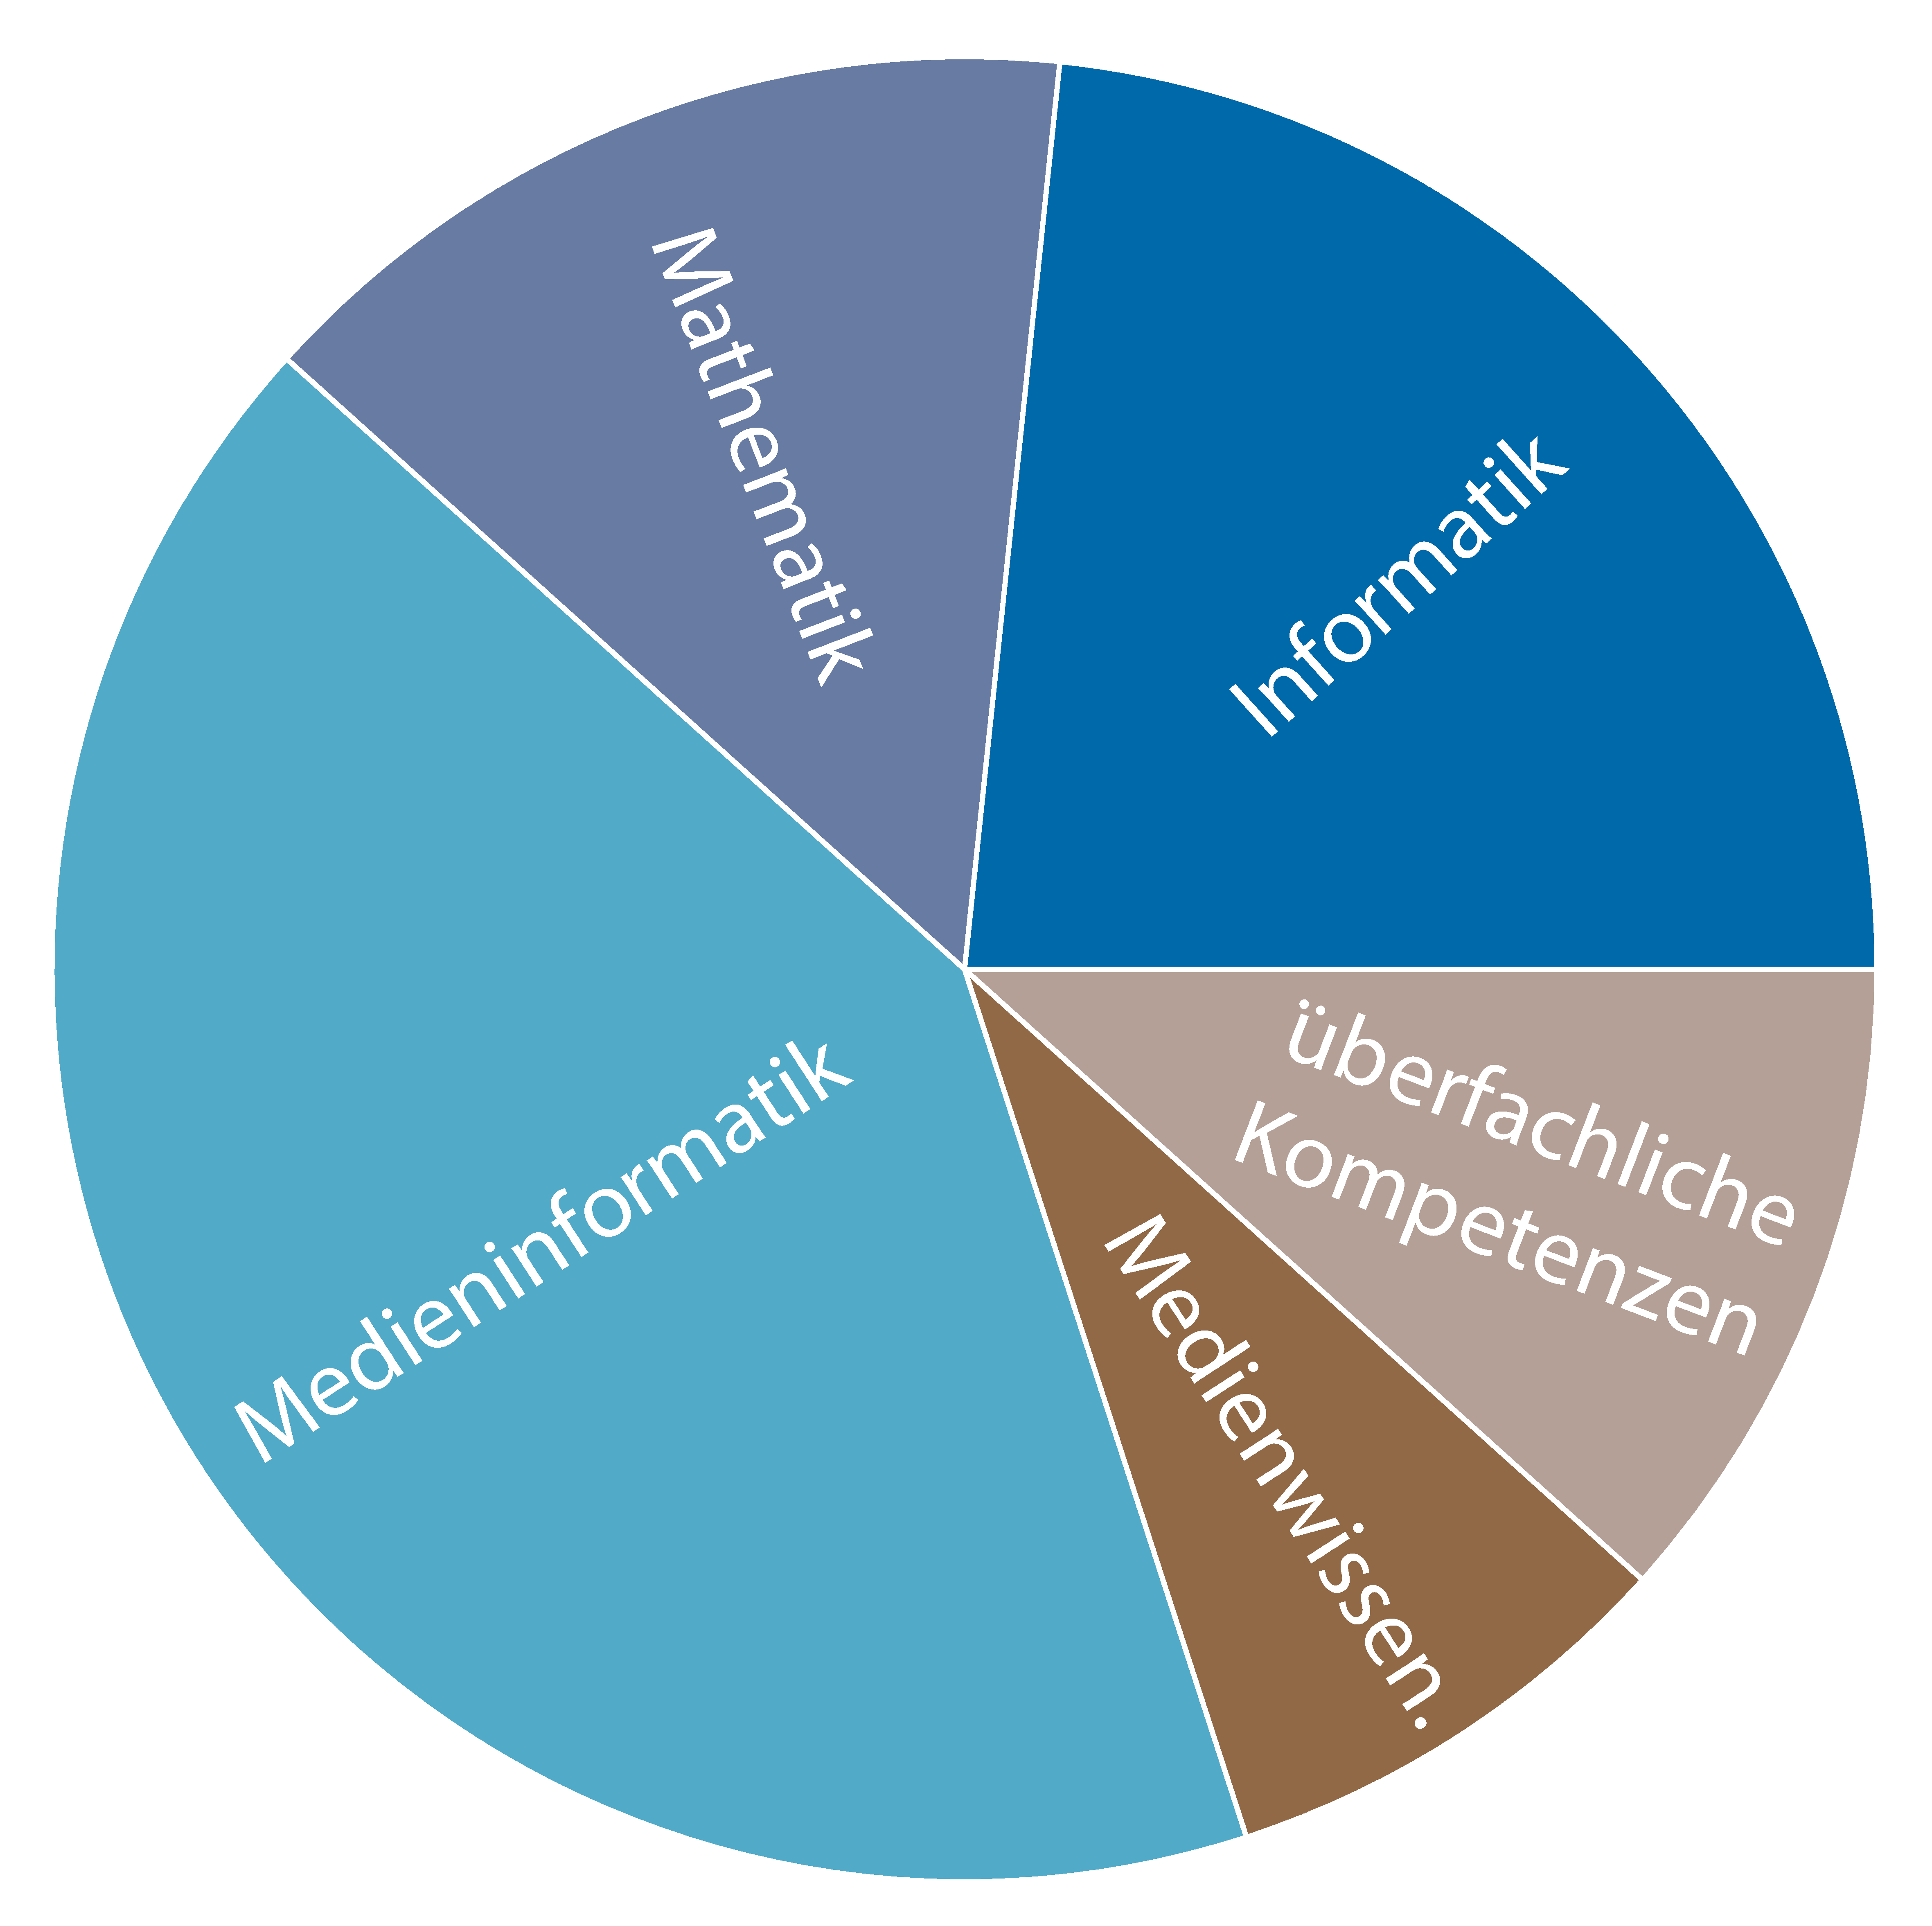
\includegraphics[width=0.4\textwidth]{charts/medieninformatik-Piechart.pdf}
			\caption{Verteilung der Themenbereiche über das komplette Studium}
		\end{figure}
	\end{block}
	\begin{block}{Was macht man in welchem Semester?}
		\begin{figure}[h!]
			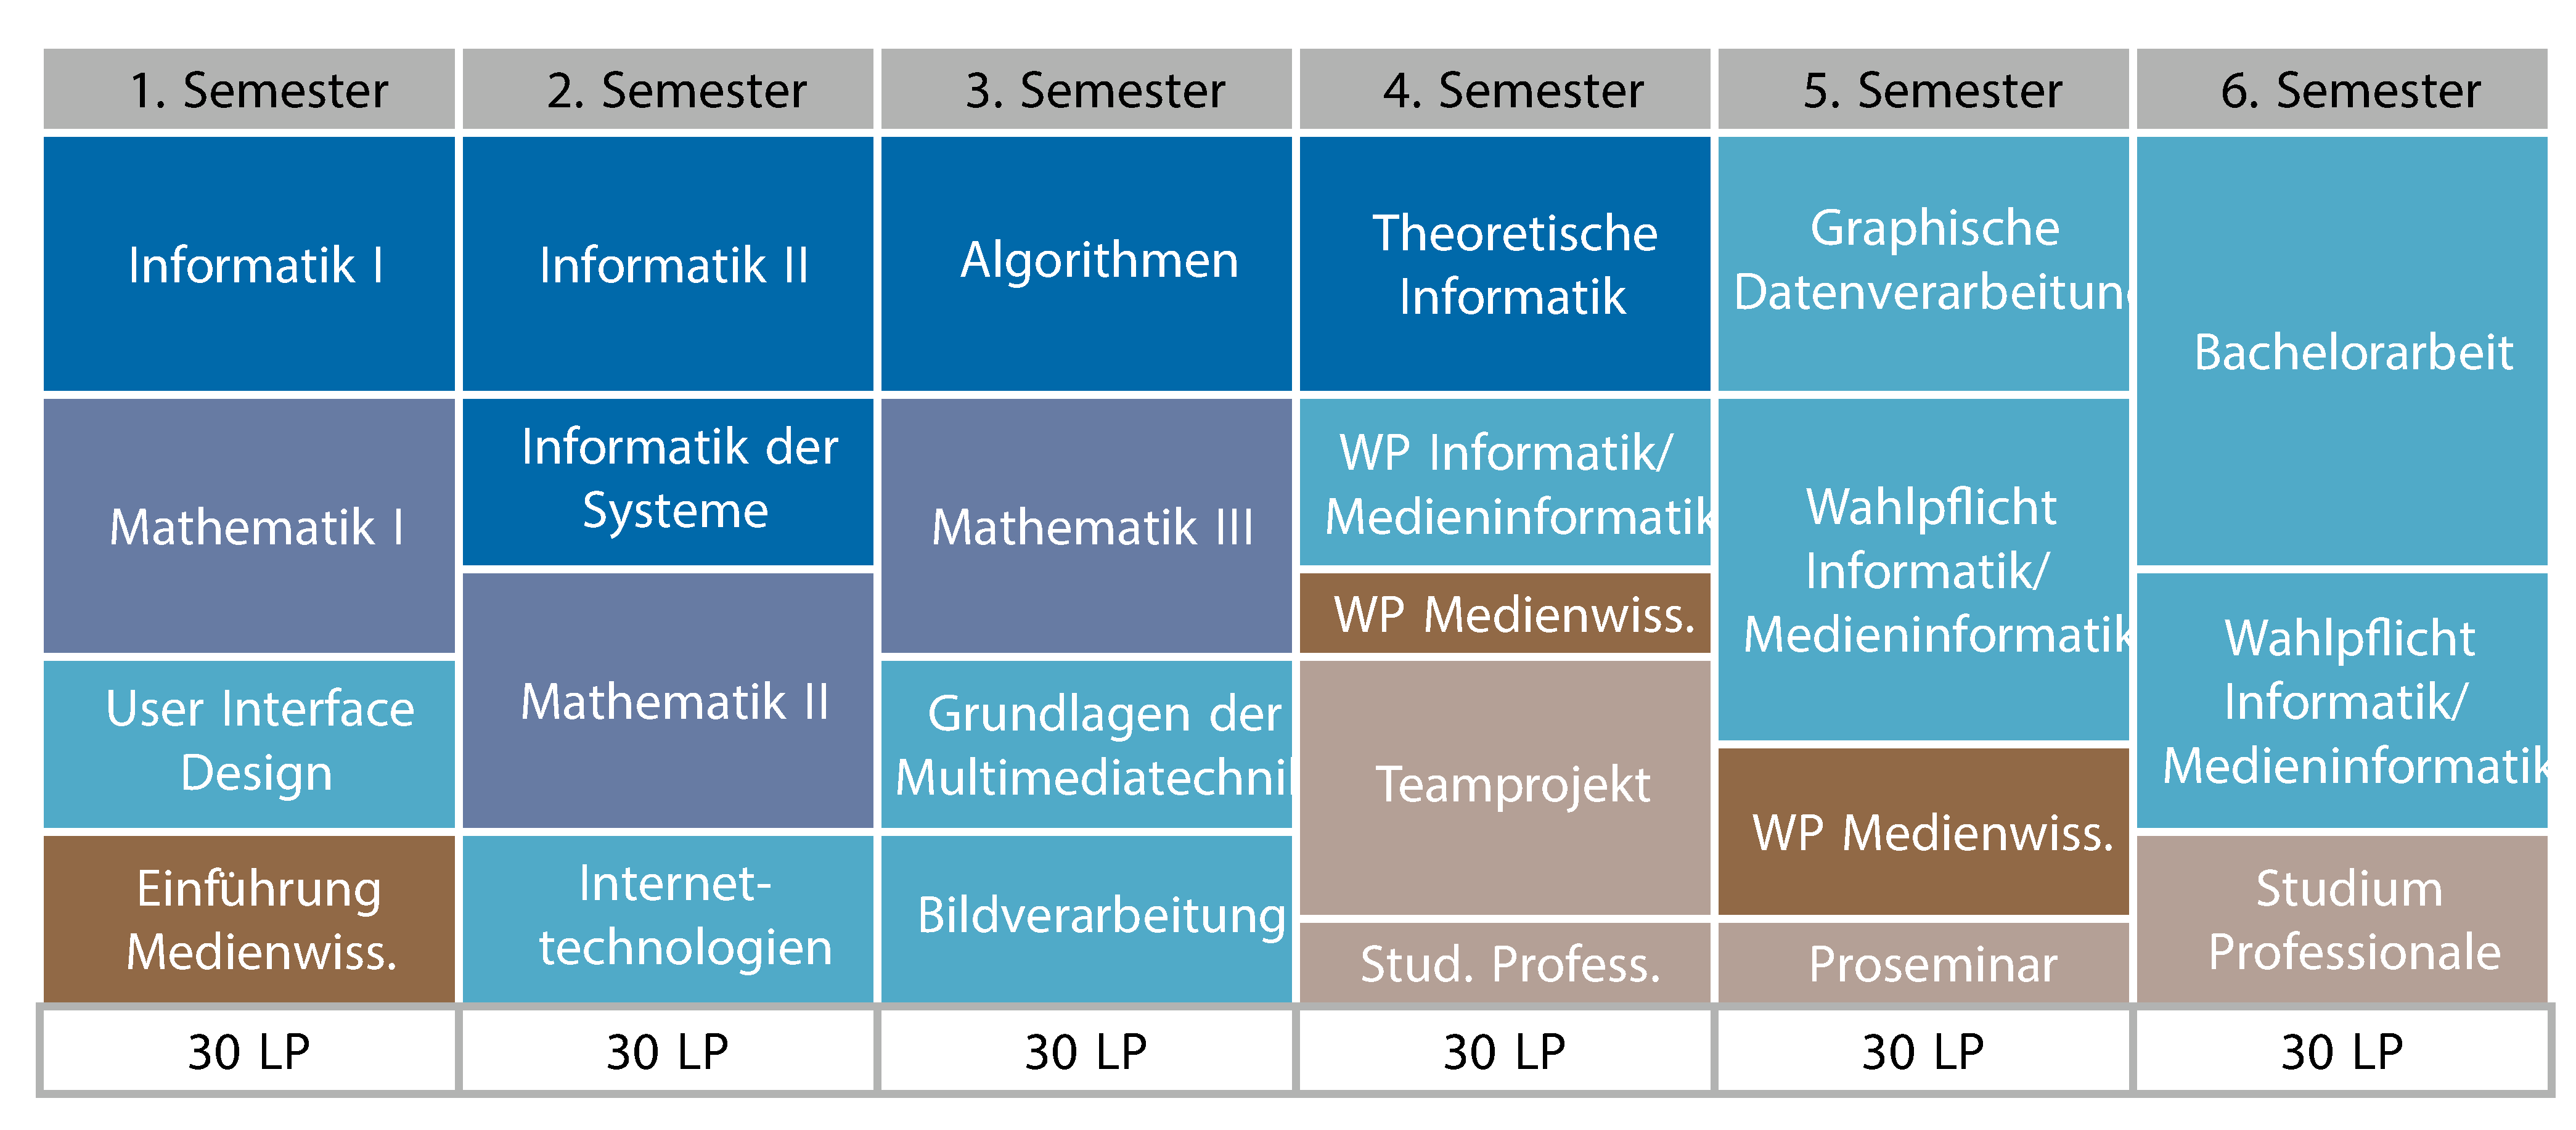
\includegraphics[width=\textwidth]{charts/medieninformatik-Studienplan_abWS18.pdf}
		\end{figure}
		Das 1. Semester ist nach Plan ein Wintersemester, der Studienbeginn ist hier auch nur zum Wintersemester möglich. 
		Dieser Verlauf ist lediglich ein Vorschlag und kein bindender Studienplan. Es empfiehlt sich jedoch, den Plan einzuhalten, wenn man in Regelstudienzeit studieren möchte.
	\end{block}
\vfill
\begin{flushright}
	\includegraphics[width=0.4\textwidth]{fsilogo.pdf}
\end{flushright}
    \column[T]{0.45\textwidth}
    \colorlet{biologie}{andere}
\colorlet{physik}{andere}
\DTLsetpiesegmentcolor{1}{info}
\DTLsetpiesegmentcolor{2}{mathe}
\DTLsetpiesegmentcolor{3}{medizininfo}
\DTLsetpiesegmentcolor{4}{andere}
\DTLsetpiesegmentcolor{5}{sq}

\begin{Huge}
    Medizininformatik
\end{Huge}

\begin{exampleblock}{\textcolor{white}{Was ist der Studiengang?}}
    Die Schnittstelle zwischen Klinikum, Ärzten und Medizintechnikern. Klassische Anwendungsbereiche sind E-Health, Medizinische Datenverarbeitung sowie die (Mit-)Entwicklung von Medizingeräten. Es wird ein stärkerer Fokus auf Biologie, Physik und medizinische Inhalte gelegt. Ein Schwerpunktfach gibt es nicht. Danach kann das Studium mit einem Master \\ (4 Semester Regelstudienzeit) weitergeführt werden.
\end{exampleblock}

\begin{block}{Welcher Teil macht wie viel im Studium aus?}
    \begin{figure}[h!]
        \vspace{-20pt}
        \begin{minipage}{\linewidth}
            \centering
            \DTLloaddb{LPverteilungMedizin}{inhalte/medizininfo.csv}
            \tikzstyle{every node}=[text width={},minimum height=0pt]
            \DTLpiechart{
                variable=\lp,
                innerlabel={\parbox{40pt}{\centering\color{white} \bereich}},
                innerratio=0.25,
                radius=70pt,
                rotateinner}{LPverteilungMedizin}{\bereich=Bereich,\lp=LP}
        \end{minipage}
        \vspace{-20pt}
        \caption{Verteilung der Themenbereiche über das komplette Studium}
    \end{figure}
\end{block}

\begin{block}{Was macht man in welchem Semester?}
    \vspace{-10pt}
    \begin{figure}[h!]
        \resizebox{\linewidth}{!}{
        \begin{minipage}{\textwidth}
            \begin{tikzpicture}
                \begin{scope}[start chain=going below,node distance=\nodedistancecorrection]
                    \semester{1}
                    \veranstaltung{9}{Praktische In\-for\-ma\-tik~1}{info}
                    \veranstaltung{9}{Mathe\-matik f. Informatik~1}{mathe}
                    \veranstaltung{6}{Grundlagen der Medizininformatik}{medizininfo}
                    \veranstaltung{3}{Humanbiologie I}{biologie}
                    \veranstaltung{3}{Med. Terminologie}{biologie}
                    \SumLP{30}
                \end{scope}
                \begin{scope}[xshift=1\lpwidth,start chain=going below,node distance=\nodedistancecorrection]
                    \semester{2}
                    \veranstaltung{9}{Praktische In\-for\-ma\-tik~2}{info}
                    \veranstaltung{6}{Einf. Internet\-technologien}{info}
                    \veranstaltung{9}{Mathe\-matik f. Informatik~2}{mathe}
                    \veranstaltung{6}{Humanbiologie II}{biologie}
                    \SumLP{30}
                \end{scope}
                \begin{scope}[xshift=2\lpwidth,start chain=going below,node distance=\nodedistancecorrection]
                    \semester{3}
                    \veranstaltung{6}{User Experience}{info}
                    \veranstaltung{6}{Praktische Informatik 3}{info}
                    \veranstaltung{6}{Physik I}{physik}
                    \veranstaltung{6}{Humanbiologie III}{biologie}                
                    \veranstaltung{3}{Biostatistik}{biologie}                
                    \veranstaltung{3}{Ethik (übK)}{sq}
                    \SumLP{30}
                \end{scope}
                \begin{scope}[xshift=3\lpwidth,start chain=going below,node distance=\nodedistancecorrection]
                    \semester{4}                
                    \veranstaltung{9}{Grundlagen Bioinformatik}{medizininfo}
                    \veranstaltung{6}{Physik II}{physik}                
                    \veranstaltung{6}{Humanbiologie IV}{biologie}
                    \veranstaltung{9}{Team\-projekt}{sq}                
                    \SumLP{30}
                \end{scope}
                \begin{scope}[xshift=4\lpwidth,start chain=going below,node distance=\nodedistancecorrection]
                    \semester{5}
                    \veranstaltung{6}{WP Informatik}{info}
                    \veranstaltung{6}{Medizinische Visualisierung}{medizininfo}
                    \veranstaltung{6}{Telemedizin}{medizininfo}
                    \veranstaltung{6}{WP Medizin/Biologie}{biologie}
                    \veranstaltung{3}{Proseminar}{sq}
                    \veranstaltung{3}{übK}{sq}
                    \SumLP{30}
                \end{scope}
                \begin{scope}[xshift=5\lpwidth,start chain=going below,node distance=\nodedistancecorrection]
                    \semester{6}
                    \veranstaltung{6}{WP Bioinformatik}{medizininfo}
                    \veranstaltung{6}{WP Medizininformatik}{medizininfo}
                    \veranstaltung{15}{Bachelor\-arbeit}{medizininfo}
                    \veranstaltung{3}{übK}{sq}
                    \SumLP{30}
                \end{scope}
            \end{tikzpicture}
        \end{minipage}}
    \end{figure}
    
    Das 1. Semester ist nach Plan ein Wintersemester, der Studienbeginn ist hier auch nur zum Wintersemester möglich. 
    Dieser Verlauf ist lediglich ein Vorschlag und kein bindender Studienplan. Es empfiehlt sich jedoch, den Plan einzuhalten, wenn man in Regelstudienzeit studieren möchte.
\end{block}

\vfill
\begin{flushright}
    \includegraphics[width=0.4\textwidth]{images/fsilogo.pdf}
\end{flushright}

\end{columns}
\newpage 
%% BLATT 2 RÜCKSEITE
%% Medizininfo und Medieninfo FAQ
%% Absichtlich falschrum!
\begin{columns}
    \column[T]{0.45\textwidth}
    \begin{Huge}
    Medizininformatik-FAQ
\end{Huge}

\begin{block}{Häufig gestellte Fragen zum Studium}

\question{Lernt man im Studium, wie man programmiert?}{
    Ja, aber auf einer sehr eigenständigen Basis. Man bekommt eine Überblick über die Sprache(n), alles andere was darüber hinaus geht muss man sich selbst aneignen.
}
\question{Welche Programmiersprachen macht man da so?}{
    Ist vom Professor abhängig. In den ersten beiden Semestern meistens entweder Java oder Racket, manchmal auch C++.
}
\question{Muss man programmieren können, um das Studium anzufangen?}{
    Nein. Die Vorlesung beginnt absolut bei 0, um allen den Einstieg zu ermöglichen.
}

\question{Muss man gut in Mathe sein?}{
    Man muss kein Mathe-Genie sein, man sollte Mathe aber nicht hassen. Es ist gerade am Anfang viel Mathe.
}
\question{Ich will eigentlich Medizin studieren, aber mein NC reicht nicht. Medizininformatik ist doch auch was mit Medizin, oder?}{
    Nein! Man lernt zwar Grundlagen der Anatomie, Histologie und Pathologie, das ist aber keinesfalls Niveau der Medizin und ihr habt auch keinen Kontakt mit Medizinern. Zweck dieser Vorlesungen ist, am Ende so ungefähr zu verstehen wovon der Mediziner redet.
}

\question{Wie ist die Frauenquote so?}{
    60\%.
}
\question{Was ist der Unterschied zwischen Bio- und Medizininformatik?}{
    Die Bioinformatik beschäftigt sich grob gesagt mit auotmatisierter Verarbeitung von DNA, Molekülstrukturen etc., Medizininformatik geht mehr in Richtung Patientendaten und medizinische Bildverarbeitung.
}
\question{Gibt es Praktika?}{
    Im normalen Studienverlauf ist kein berufsorientiertes Praktikum vorgesehen, viele arbeiten aber parallel als Werksstudent oder man macht ein Kurzpraktikum in den Semesterferien.
}

\question{Kann man ein Auslandssemester machen?}{
    Klar, geht immer. Tübingen nimmt am ERASMUS-Programm teil, die Organisation ist aber langwierig und man sollte sich früh drum kümmern.
}

\question{Was arbeitet man danach so?}{
    Alle Bereiche der IT-Branche, insbesondere in den vielfältigen Berufsfeldern der medizinischen Informationsverarbeitung und des Gesundheitswesens.
}

\question{Wie ist da so der NC?}{
    2,8 (WS 2018/19). Das muss aber in den nächsten Jahren nicht zwingend noch so sein, der Wert ändert sich hier relativ rasch nach oben.
}
\end{block}

    \column[T]{0.45\textwidth}
    \begin{Huge}
	Medieninformatik-FAQ
\end{Huge}
\begin{block}{Häufig gestellte Fragen zum Studium}
\begin{large}
\begin{itemize}
		\item \textbf{Lernt man im Studium, wie man programmiert?}
		\begin{itemize}
			\item Ja, aber auf einer sehr eigenständigen Basis. Man bekommt eine Überblick über die Sprache(n), alles andere was darüber hinaus geht muss man sich selbst aneignen.
		\end{itemize}
	
		\item \textbf{Welche Programmiersprachen macht man da so?}
		\begin{itemize}
			\item Ist vom Professor abhängig. In den ersten beiden Semestern meistens entweder Java oder Racket, manchmal auch C++.
		\end{itemize}
	
		\item \textbf{Muss man programmieren können, um das Studium anzufangen?}
		\begin{itemize}
			\item Nein. Die Vorlesung beginnt absolut bei 0, um allen den Einstieg zu ermöglichen.
		\end{itemize}
	
		\item \textbf{Muss man gut in Mathe sein?}
		\begin{itemize}
			\item Man muss kein Mathe-Genie sein, man sollte Mathe aber nicht hassen. Es ist gerade am Anfang viel Mathe.
		\end{itemize}

	\item \textbf{Ich mache voll gerne Design und so, kann ich Medieninformatik studieren?}
	\begin{itemize}
		\item Medieninformatik ist vor allem eines: Informatik. Gestaltung von Nutzeroberflächen gehört zwar zum Studium dazu, ist aber nur ein Teilgebiet. Der andere Teil ist: viel programmieren, viel Mathe.
	\end{itemize}

\item \textbf{Ich kann schon Photoshop, bringt mir das bei Medieninformatik was?}
\begin{itemize}
	\item Nein.
\end{itemize}

\item \textbf{Wie ist die Frauenquote so?}
\begin{itemize}
	\item 27\%.
\end{itemize}

\item \textbf{Lerne ich im Studium, wie man Webseiten baut?}
\begin{itemize}
	\item In einer Veranstaltung, ja. Die ersten ca. 3 Semester haben viel mit Web und User-Interfaces zu tun, danach verschiebt sich der Schwerpunkt je nach persönlicher Präferenz.
\end{itemize}

\item \textbf{Lerne ich, wie man Computerspiele baut?}
\begin{itemize}
	\item Die Möglichkeit besteht, ist aber nicht grundlegender Teil des Studiums und kommt, wenn überhaupt, erst im dritten Studienjahr oder später.
\end{itemize}

\item \textbf{Was arbeitet man danach so?}
\begin{itemize}
	\item alle Bereiche der IT-Branche, insbesondere Webentwicklung, Entwicklung von Computerspielen, in der Filmindustrie, Automobilbranche und Medizintechnik.
\end{itemize}

\item \textbf{Gibt es Praktika?}
\begin{itemize}
	\item Im normalen Studienverlauf ist kein berufsorientiertes Praktikum vorgesehen, viele arbeiten aber parallel als Werksstudent oder man macht ein Kurzpraktikum in den Semesterferien.
\end{itemize}

\item \textbf{Kann man ein Auslandssemester machen?}
\begin{itemize}
	\item Klar, geht immer. Tübingen nimmt am ERASMUS-Programm teil, die Organisation ist aber langwierig und man sollte sich früh drum kümmern.
\end{itemize}

\item \textbf{Wie ist da so der NC?}
\begin{itemize}
	\item 2,7 (WS18/19). Das muss aber in den nächsten Jahren nicht zwingend noch so sein, der Wert ändert sich immer.
\end{itemize}

\end{itemize}

\end{large}
\end{block}		
\end{columns}
\newpage 
%% BLATT 3 VORDERSEITE
%% Kogni und Lehramt Infotexte
\begin{columns}
    \column[T]{0.45\textwidth}
    \colorlet{other}{brown}
\colorlet{philo}{other}
\colorlet{lingu}{other}
\colorlet{neuro}{other}
\colorlet{psycho}{other}
\colorlet{bscarb}{other}


\DTLsetpiesegmentcolor{1}{kogni}
\DTLsetpiesegmentcolor{2}{info}
\DTLsetpiesegmentcolor{3}{mathe}
\DTLsetpiesegmentcolor{4}{other}
\DTLsetpiesegmentcolor{5}{sq}

\begin{Huge}
    Kognitionswissenschaft
\end{Huge}

\begin{exampleblock}{\textcolor{white}{Was ist der Studiengang?}}
    Ein sehr interdisziplinärer Studiengang, der einzelne Aspekte der Informatik, (Neuro-)Biologie, Linguistik, Philosophie und Psychologie miteinander verbindet, bzw. auch einzeln behandelt. Alle Fragen, die dem Denken gewidmet sind, finden hier ihren Platz und werden mithilfe der verschiedenen Sichtweisen der unterschiedlichen Disziplinen versucht zu beantworten. Ein Schwerpunktfach gibt es nicht. Danach kann das Studium mit einem Master (4 Semester Regelstudienzeit) weitergeführt werden.
\end{exampleblock}

\begin{block}{Welcher Teil macht wie viel im Studium aus?}
    \begin{figure}[h!]
        \vspace{-10pt}
        \begin{minipage}{\linewidth}
            \centering
            \DTLloaddb{LPverteilungKogni}{inhalte/kogni.csv}
            \tikzstyle{every node}=[text width={},minimum height=0pt]
            \DTLpiechart{
                variable=\lp,
                innerlabel={\parbox{40pt}{\centering\color{white} \bereich}},
                innerratio=0.25,
                radius=70pt,
                rotateinner}{LPverteilungKogni}{\bereich=Bereich,\lp=LP}
        \end{minipage}
        \vspace{-20pt}
        \caption{Verteilung der Themenbereiche über das komplette Studium}
    \end{figure}
\end{block}

\begin{block}{Was macht man in welchem Semester?}
    \vspace{-10pt}
    \begin{figure}[h!]
        \resizebox{\linewidth}{!}{
        \begin{minipage}{\textwidth}
            \begin{tikzpicture}
                \begin{scope}[start chain=going below,node distance=\nodedistancecorrection]
                    \semester{1}
                    \veranstaltung{9}{In\-for\-ma\-tik~I}{info}
                    \veranstaltung{9}{Mathe\-matik f. Informatik~I}{mathe}        
                    \veranstaltung{6}{Neuro\-bio\-logie und Sinnes\-physio\-logie}{neuro}
                    \veranstaltung{3}{Mathem. Statistik I}{kogni}
                    \veranstaltung{3}{Einf.\ Kognition}{kogni}
                    \SumLP{30}
                \end{scope}
                \begin{scope}[xshift=1\lpwidth,start chain=going below,node distance=\nodedistancecorrection]
                    \semester{2}
                    \veranstaltung{9}{In\-for\-ma\-tik~II}{info}
                    \veranstaltung{9}{Mathe\-matik f. Informatik~II}{mathe}
                    \veranstaltung{3}{Allg. Psych. C}{psycho}
                    \veranstaltung{3}{Comp. Statistik}{kogni}
                    \veranstaltung{3}{Statistik II}{kogni}
                    \veranstaltung{3}{Forschungsmeth.}{kogni}
                    \SumLP{30}
                \end{scope}
                \begin{scope}[xshift=2\lpwidth,start chain=going below,node distance=\nodedistancecorrection]
                    \semester{3}
                    \veranstaltung{9}{Al\-go\-rith\-men}{info}
                    \veranstaltung{9}{Mathe\-matik f. Informatik~III}{mathe}
                    \veranstaltung{6}{Linguistik}{lingu}
                    \veranstaltung{6}{Exp. Kogwiss.}{kogni}
                    \veranstaltung{3}{Allg. Psych. B}{psycho}
                    \SumLP{33}
                \end{scope}
                \begin{scope}[xshift=3\lpwidth,start chain=going below,node distance=\nodedistancecorrection]
                    \semester{4}     
                    \veranstaltung{9}{Team\-projekt}{sq}
                    \veranstaltung{6}{Philosophie}{philo}
                    \veranstaltung{6}{Language \& Cogn.}{lingu}
                    \veranstaltung{3}{Kog. Architekturen}{kogni}
                    \veranstaltung{3}{Psychologie}{psycho}
                    \SumLP{27}
                \end{scope}
                \begin{scope}[xshift=4\lpwidth,start chain=going below,node distance=\nodedistancecorrection]
                    \semester{5}
                    \veranstaltung{6}{Kognitions\-informatik}{info}
                    \veranstaltung{6}{Computational Neuroscience}{neuro}
                    \veranstaltung{12}{Vertiefung Kogwiss.}{kogni}
                    \veranstaltung{3}{Forschungsseminar}{kogni}
                    \veranstaltung{3}{Psychologie}{psycho}
                    \SumLP{30}
                \end{scope}
                \begin{scope}[xshift=5\lpwidth,start chain=going below,node distance=\nodedistancecorrection]
                    \semester{6}
                    \veranstaltung{15}{Bachelor\-arbeit}{kogni}
                    \veranstaltung{9}{Studium Professionale}{sq}
                    \veranstaltung{3}{Forschungsseminar}{kogni}
                    \veranstaltung{3}{Kolloquium}{sq}
                    \SumLP{30}
                \end{scope}
            \end{tikzpicture}
        \end{minipage}}        
    \end{figure}

    Das 1. Semester ist nach Plan ein Wintersemester, der Studienbeginn ist hier auch nur zum Wintersemester möglich. 
    Dieser Verlauf ist lediglich ein Vorschlag und kein bindender Studienplan. Es empfiehlt sich jedoch, den Plan einzuhalten, wenn man in Regelstudienzeit studieren möchte.
\end{block}

\vfill
\begin{flushright}
    \includegraphics[width=0.4\textwidth]{images/fsilogo.pdf}
\end{flushright}

    \column[T]{0.45\textwidth}
    	\begin{Huge}
			Informatik (Bachelor of Education)
		\end{Huge}
		\begin{exampleblock}{\textcolor{white}{Was ist der Studiengang?}}
			
		\end{exampleblock}
	
	\begin{block}{Welcher Teil macht wie viel im Studium aus?}
		\begin{figure}[h!]
			\includegraphics[width=0.4\textwidth]{charts/lehramt_informatik_piechartonly.pdf}
			\caption{Verteilung der Themenbereiche über das komplette Studium}
		\end{figure}
	\end{block}
	
	\begin{block}{Was macht man in welchem Semester?}
		\begin{figure}[h!]
			\includegraphics[width=\textwidth]{charts/lehramt_informatik_Studienplanonly.pdf}
			\caption{Vorschlag für den Studienverlauf}
		\end{figure}
		Dieser Verlauf ist allerdings nur ein Vorschlag und kein bindender Studienplan.
	\end{block}

\end{columns}
\newpage 
%% BLATT 3 RÜCKSEITE
%% Lehramt und Kogni FAQ
%% Absichtlich falschrum!
\begin{columns}
    \column[T]{0.45\textwidth}
    \begin{Huge}
    Informatik (Bachelor of Education)-FAQ
\end{Huge}

\begin{block}{Häufig gestellte Fragen zum Studium}

\question{Lernt man im Studium, wie man programmiert?}{
    Ja, aber auf einer sehr eigenständigen Basis. Man bekommt eine Überblick über die Sprache(n), alles andere was darüber hinaus geht muss man sich selbst aneignen.
}

\question{Welche Programmiersprachen macht man da so?}{
    Ist vom Professor abhängig. In den ersten beiden Semestern meistens entweder Java oder Racket, manchmal auch C++.
}

\question{Muss man programmieren können, um das Studium anzufangen?}{
    Nein. Die Vorlesung beginnt absolut bei 0, um allen den Einstieg zu ermöglichen.
}

\question{Muss man gut in Mathe sein?}{
    Man muss kein Mathe-Genie sein, man sollte Mathe aber nicht hassen. Auch wenn man nur Mathe I hat, benötigt man für die Informatik einiges an mathematischer Denkweise.
}

\question{Welche Fächer kann man mit Informatik kombinieren?}{
    Alles außer NWT.
}

\question{Was, wenn ich merke, dass Lehramt doch nichts für mich ist?} {
    Du kannst Informatik gegen ein anderes Fach tauschen oder dich vom B.Ed. verabschieden und auf ein "`normales"' B.Sc.-Studium wechseln.
}

\question{Was mache ich denn mit einem Bachelor of Education?} {
    Die kurze Antwort: Weiter machen. Der Bachelor ist nur ein Teil deines Lehramtsstudiums, danach folgen noch der Master und das Referendariat.
}

\question{Wie sind meine Berufsschancen?} {
    Da in BaWü ein großer Informatiklehrermangel herrscht, sind deine Berufschancen sehr hoch.
}

\question{Was ist denn der Unterschied zwischen B.Sc. und B.Ed?} {
    Im B.Ed. hört man ein paar weniger Informatikvorlesungen als im B.Sc. und hat dafür Vorlesungen zu Bildungswissenschaften und Fachdidaktik.
}

\question{Was ist Fachdidaktik?} {
    In Fachdidaktik lernt man, wie man sein Wissen SuS~ (Schülerinnen und Schülern) beibringt und wie man Unterricht am besten planen kann.
}

\question{Gibt es Praktika?}{
    Ja, nachdem du BWS-I bestanden hast, musst du ein dreiwöchiges Orientierungspraktikum an der Schule machen, das in den Semesterferien stattfindet. Man hat zum Ablegen dieses Praktikums aber bis zum Ende des Bachelors Zeit. Im Master gibt es dann noch ein komplettes Semester Schulpraxis.
}

\question{Wie ist da so der NC?}{
    Gibt es keinen.
}

\question{In welchen Klassenstufen wird Informatik unterrichtet?}{
    Hier ein kleines Schaubild zur Erläuterung, wie es eigentlich sein sollte:
    \begin{figure}[h!]
        \vspace{-1em}
        \includegraphics[width=0.6\linewidth]{images/info_bed_klassenstufen.png}
        \vspace{-1em}
    \end{figure}
    Momentan ist es aber leider so, dass sich Schulen aufgrund des Lehrermangels kaum an diesen Lehrplan halten können.
}
\end{block}

    \column[T]{0.45\textwidth}
    \begin{Huge}
    Kognitionswissenschaft-FAQ
\end{Huge}

\begin{block}{Häufig gestellte Fragen zum Studium}

\question{Lernt man im Studium, wie man programmiert?}{
    Ja, aber auf einer sehr eigenständigen Basis. Man bekommt eine Überblick über die Sprache(n), alles andere was darüber hinaus geht muss man sich selbst aneignen.
}

\question{Welche Programmiersprachen macht man da so?}{
    Ist vom Professor abhängig. In den ersten beiden Semestern meistens entweder Java oder Racket, manchmal auch C++.
}

\question{Muss man programmieren können, um das Studium anzufangen?}{
    Nein. Die Vorlesung beginnt absolut bei 0, um allen den Einstieg zu ermöglichen.
}

\question{Muss man gut in Mathe sein?}{
    Man muss kein Mathe-Genie sein, man sollte Mathe aber nicht hassen. Es ist gerade am Anfang viel Mathe.
}

\question{Was mache ich nachher damit?}{
    Eine wirklich sehr gute Frage - die nicht so einfach zu beantworten ist. Wir haben die Möglichkeit uns im Master weiter zu spezialisieren, Richtung Informatik, Biologie oder was sonst noch so grob passt. Davon hängt dann auch sehr stark die spätere Berufsaussicht ab. Reine Kognitionswissenschaft findet man vor allem in der Forschung, ein weiteres großes Feld ist Maschinelles Lernen, bzw. Künstliche Intelligenz.
}

\question{Wie ist die Frauenquote so?}{
    55\%.
}

\question{Ich kenne mich mit Informatik gar nicht aus. Ist das schlimm?}{
    Nein, ist es nicht. Wenn du einigermaßen logisch denken kannst und dir auch Mathe ganz gut liegt, dann kriegst du das auch hin.
}

\question{Eigentlich will ich ja Psychologie studieren, aber mein NC reicht nicht. Kogni ist doch auch was mit Psychologie, oder?}{
    Schon, ja. Allerdings ist der Anteil im Bachelor-Studiengang nicht allzu hoch. Besonders am Anfang sind größere Schwerpunkte Informatik und Mathe, das sollte man auf jeden Fall mit in Betracht ziehen. Im weiteren Verlauf des Studiums kann man sich aber weiter in Richtung Psychologie vertiefen.
}

\question{Kann ich danach auf Psychologie wechseln?}{
    Das können wir so allgemein nicht beantworten. Generell hängt das sehr stark von der Uni ab, an der man studieren möchte. Das müsste man dann im Zweifelsfall vorher schon mal anfragen.
}

\question{Gibt es Praktika?}{
    Im normalen Studienverlauf ist kein berufsorientiertes Praktikum vorgesehen, viele arbeiten aber parallel als Werksstudent oder man macht ein Kurzpraktikum in den Semesterferien.
}

\question{Kann man ein Auslandssemster machen?}{
    Klar, geht immer. Tübingen nimmt am ERASMUS-Programm teil, die Organisation ist aber langwierig und man sollte sich früh (ein Jahr vorher) drum kümmern.
}

\question{Wie ist da so der NC?}{
    1,9 (WS22/23). Das muss aber in den nächsten Jahren nicht zwingend noch so sein, der Wert ändert sich immer.
}
\end{block}
		
\end{columns}
\end{document}
